% simple.tex - A simple article to illustrate document structure.

% Andrew Roberts - June 2003

\documentclass[10pt, a4paper,notitlepage]{article}
\usepackage[spanish]{babel}%Para el español
\usepackage[utf8]{inputenc}


%\usepackage{times}
\usepackage{color}
\usepackage[dvipsnames]{xcolor}
\usepackage{listings}
\usepackage{textcomp}
\usepackage{pdfpages}

\usepackage{verbatim}

\usepackage{amsmath}
\usepackage{courier} %--lisitngs
\usepackage{mathptmx} %-->TimesNewRoman

\usepackage{caption}
\DeclareCaptionFont{white}{\color{white}}
\definecolor{dark-gray}{cmyk}{0,0,0,0.7}
\DeclareCaptionFormat{listing}{\colorbox{dark-gray}{\parbox{\textwidth}{#1#2#3}}}
\captionsetup[lstlisting]{format=listing,labelfont={white,sf},textfont={white,sf}}

\usepackage{graphicx} % Required for including pictures

\usepackage{float} % Allows putting an [H] in \begin{figure} to specify the exact location of the figure
\usepackage{wrapfig} % Allows in-line images such as the example fish picture
\graphicspath{{Imagenes/}} % Specifies the directory where pictures are stored

\usepackage{xcolor}
\definecolor{lbcolor}{rgb}{0.9,0.9,0.9}
\lstset{
backgroundcolor=\color{gray!20!white},
    tabsize=2,
    literate=%
	{á}{{\'{a}}}1
    {é}{{\'{e}}}1
    {í}{{\'{i}}}1
    {ó}{{\'{o}}}1
    {ú}{{\'{u}}}1
    {ñ}{{\~{n}}}1
    {<}{{$<$}}1
    {>}{{$>$}}1,
%   rulecolor=,
    %language=C,
    %language=bash,
    		linewidth=12.2cm,
		belowcaptionskip=0.1\baselineskip,
		xleftmargin=\parindent,        
        %basicstyle=\scriptsize,
        basicstyle=\footnotesize\bfseries\ttfamily\color{black!80!white},
        upquote=true,
        %aboveskip={1.5\baselineskip},
        columns=fixed,
        showstringspaces=false,
        extendedchars=false,
        breaklines=true,
        prebreak = \raisebox{0ex}[0ex][0ex]{\ensuremath{\hookleftarrow}},
	%frame=lines,
        numbers=left,
        showtabs=false,
        showspaces=false,
        showstringspaces=false,
        identifierstyle=\ttfamily,
        commentstyle=\color{orange!80!black},
        keywordstyle=\bfseries\color[rgb]{0,0,1},
        %commentstyle=\bfseries\color[rgb]{0.026,0.112,0.095},
        %stringstyle=\bfseries\color[rgb]{0.627,0.126,0.941},
        stringstyle=\bfseries\color{green!50!black},
        numberstyle=\ttfamily\color[rgb]{0.205, 0.142, 0.73},
%        \lstdefinestyle{C++}{language=C++,style=numbers}’.
}
\lstdefinelanguage{linux_bash}
{ language=bash,%-->me baso en bash
alsoletter={-},%-->me habilita (-) en medio de los keywords
morekeywords={sudo,nano,apt-get,cd,ls,ln,mkdir,ifconfig,cp,wget,ppa:,add-apt-repository,install,a2ensite,service,curl},
%sensitive=false,
}
\lstdefinelanguage{cisco}
{
alsoletter={-},%-->me habilita (-) en medio de los keywords
keywords={enable,configure,terminal,interface,fastEthernet,ipv6,address,no,shutdown,route,running-config,startup-config,copy,exit,unicast-routing,brief},
%sensitive=false,
}

\renewcommand{\lstlistingname}{Código}
\renewcommand{\familydefault}{\rmdefault}
\pretolerance=2000
\tolerance=3000
\newcommand{\HRule}{\rule{\linewidth}{0.5mm}} % Defines a new command for the horizontal lines, change thickness here
\usepackage{hyperref}
\hypersetup{%
colorlinks=true,
urlcolor=blue,
urlbordercolor=blue,
pdfborderstyle={/S/U/W 1}%
}

\begin{document}

% Article top matter
{\center \large \textsf{Facultad de Ciencias Exactas, Físicas y Naturales, Progarmacion Concurrente\\}}
\title{%\HRule \\[0.4cm]		
		{ \bfseries{Trabajo Práctico Final: Sistema de manufacturación robotizado simulado mediante Redes de Petri.}}\\[0.4cm]
		%\HRule \\[1.5cm]
		} %\LaTeX is a macro for printing the Latex logo
\author{
	\textsc{Aguerreberry}, Matthew  {\small \texttt{Mat:93.739.112}}\\
	\href{mailto:mtaguerreberry@gmail.com}{mtaguerreberry@gmail.com}\\
	\textsc{Tomattis}, Natasha  {\small \texttt{Mat:38.728.783}}\\
	\href{mailto:natitomattis@gmail.com}{natitomattis@gmail.com}\\
	\textsc{Trombotto}, Agustin  {\small \texttt{Mat:12.345.678}}\\
	\href{mailto:agustin.trombotto@alumnos.unc.ed.ar}{agustin.trombotto@alumnos.unc.ed.ar}\\
}
%\affil{Facultad de Ciencias Exáctas, Físicas \& Naturales, Universidad Nacional de Córdoba, Argentina.}

%\date{\today}  %\today is replaced with the current date
%\maketitle
{\let\newpage\relax\maketitle}

\begin{par}  
\textbf{Resumen} Las Redes de Petri conforman una herramienta gráfica y matemática que puede aplicarse a cualquier sistema. Especialmente, a los sistemas paralelos que requieran simulación y modelado de la concurrencia y el uso en recursos compartidos. En este trabajo, se presenta un sistema de manufactura con estas características y se modela por medio de Redes de Petri con el objeto de analizar su dinámica y hallar la secuencia óptima de funcionamiento del sistema.
\\  
\end{par}

\textbf{Palabras Clave:} Redes de Petri, sistema de manufactura , Concurrencia, Monitor.\\
%\clearpage

\section{Introducción}
Es un elemento muy importante del paper, a través de ella el lector se nutre de la información 
suficiente para  comprender y evaluar por qué fue necesario realizar el estudio.
La introducción lleva al lector desde lo que ya sabe a lo que el investigador quiere decirle. Al
terminar de leer la introducción, el lector estará persuadido de que hay un problema
importante que abordar y comprenderá el contexto del mensaje principal que se le transmitió.
Por lo tanto, la introducción debe concentrar, con fluidez y precisión, de manera discursiva, los
principales elementos del problema y de la investigación, permitiendo al lector familiarizarse
con ellos.
He aquí una lista de aspectos que se deben tener en cuenta en la preparación de la introducción:
\begin{itemize}
	\item El tema de investigación; 
	\item El objeto de estudio; 
	\item Las motivaciones de la investigación; 
	\item La relevancia del tema; 
	\item El listado de los datos que serán recolectados y/o analizados; 
	\item La mención del o los métodos de análisis; 
	\item Panorámica general del problema que motiva la investigación; 
	\item Los resultados genéricos que se espera obtener; 
	\item Los alcances espacio-temporales de la investigación. 
\end{itemize}

Es de suma importancia señalar el propósito de la investigación, lo cual se logra simplemente 
parafraseando   el  objetivo   general,   además   de   utilizarse   el   parafraseo   de   los   objetivos 
específicos para indicar como se hizo para lograr dicho propósito.\\
También es conveniente exponer en la introducción la hipótesis de trabajo, algo así 
como: en este trabajo se estudió la influencia del tamaño del empaque en la caída de presión con lo cual 
se esperaba demostrar que esta se incrementa con la reducción del tamaño de partícula.\\
Otro ejemplo  de  hipótesis  de  trabajo  es: se  efectúa  la  evaluación  del  proceso  en  escala  de 
laboratorio y los datos recabados permitirán el diseño de un equipo a escala industrial.
No  debe  faltar  en  la  introducción  la  descripción  resumida  de  la  metodología  utilizada,  con 
énfasis en el tipo de estudio, diseño de investigación, enfoque epistemológico, identificación de 
la  población,  tipo  de  muestreo  utilizado,  tamaño  de  la  muestra,  breve  descripción  de  los 
instrumentos   de   recolección   de   datos   que   empleo,   los   resulta
dos   de   su   validación   y cuantificación de su confiabilidad, una pequeña descripción de la forma como se presentan los 
resultados y un esbozo de las conclusiones que se obtienen.

\section{Problema propuesto}
El sistema de manufacturación consiste en tres robots R1, R2 y R3 cuatro máquinas M1, M2, M3 y M4, tres tipos diferentes de piezas a procesar A, B y C, como se observa en la figura.
Las piezas provienen de tres contenedores de entrada distintos, I1, I2 e I3, de los cuales los robots las retiran, las colocan en las máquinas para su procesamiento y depositan en tres contenedores de salidas distintos, que son: O1, O2 y O3.

\begin{figure}[H] % Example image
	\centering{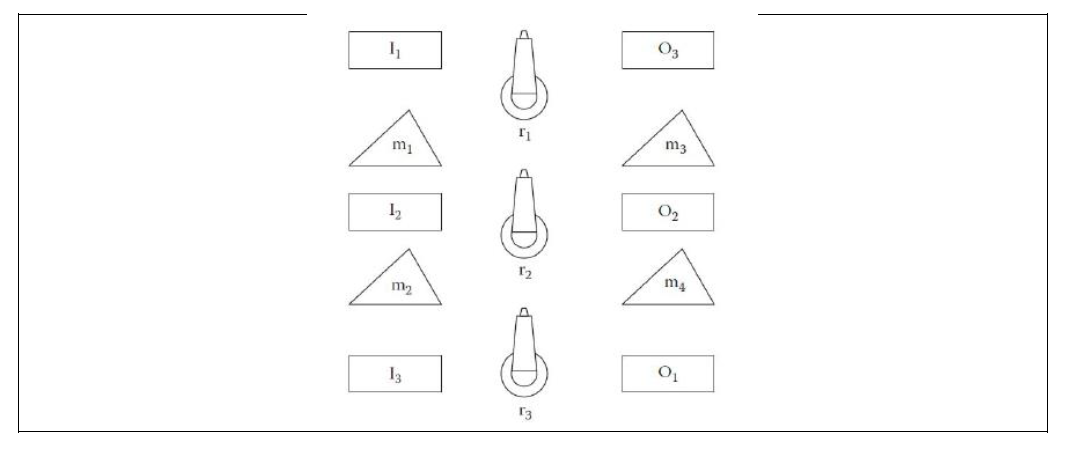
\includegraphics[width=1\linewidth]{./figure/robots.png}}
	\caption{Esquema del sistema a implementar.}
	\label{fig:I1}
\end{figure}

Adicionalmente se deberá agregar un tiempo asociado al trabajo de las maquinas, para aproximarse una aplicación en tiempo real.


\section{Solución a la red de petri}
A la presentación del problema se le adjunto una primera aproximación a una red de Petri que representa el problema, pero esta red no funciona correctamente ya que no cumple con ciertas propiedades inherentes a la concurrencia. Estas propiedades aseguran el correcto ejecución de las instrucciones del programa en paralelamente.\\
La propiedad que no se cumple en este caso es la de intrebloqueo; un problema de los sistemas concurrentes en donde todos los procesos están esperando un evento que nunca ocurrirá. Para evitar esta situación se utilizarán restricciones para que un solo hilo pueda acceder a la vez a secciones donde se puede producir interbloqueo.
\\
Se realizara la verificación de esta propiedad de la red, por medio de un software de simulación, PIPE. El cual por medio de un modelo matemático obtiene las propiedades de la Red.\\
Se propone agregar tres plazas a la red para evitar el interbloqueo:
\\
\textit{Plaza 1:}
Por medio de simulaciones de producción de una pieza única en todo el sistema, se comprobó que en el caso de la pieza B en su camino se bloqueaba cuando se intentaban producir dos piezas en el mismo camino. Esto se debe a que en la producción de esta pieza se emplea dos veces al mismo robot (R2), entones cuando una de las piezas se esta produciendo y entra otra que ocupa el robot la primera no podrá disparar la transición dado que el robot esta ocupado y la segunda no podrá disparar su transición siguiente porque la primera pieza esta usando la maquina que esta necesita.


\begin{figure}[H] % Example image
	\centering{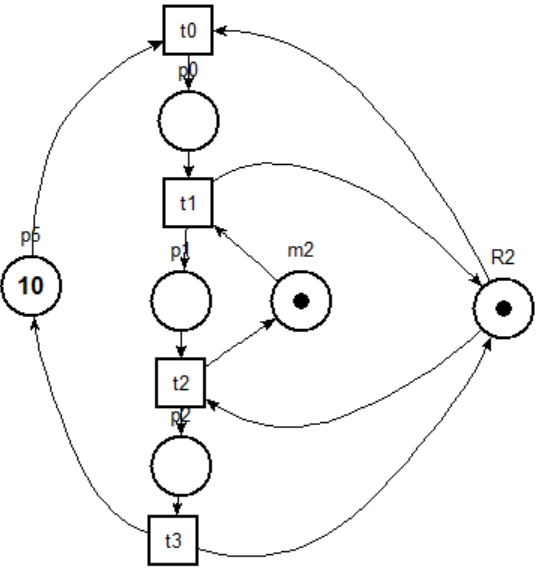
\includegraphics[width=0.4\linewidth]{./figure/I10}}
	{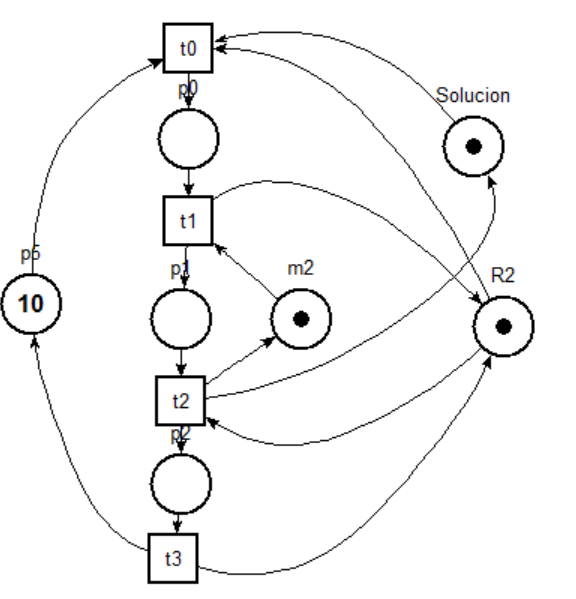
\includegraphics[width=0.4\linewidth]{./figure/I11}}
	\caption{Esquema simplificado del primer problema de interbloqueo.}
	\label{fig:I10}
\end{figure}

\textit{Plaza 2:}
Una vez finalizadas las simulaciones de la producción de piezas del mismo tipo, se procedió a realizar simulaciones de a dos piezas al mismo tiempo, dividiendo la producción de la pieza A en dos habilitando los caminos por separado. De este modo se descubrió un interbloqueo entre la linea de producción de la pieza B y uno de los caminos de la pieza A. Siendo en este caso nuevamente el robot R2 y la maquina M2 los recursos en conflicto. En este caso también se agrego una restricción para que accedan a estos recursos una linea de producción a la vez.

\begin{figure}[H] % Example image
	\centering{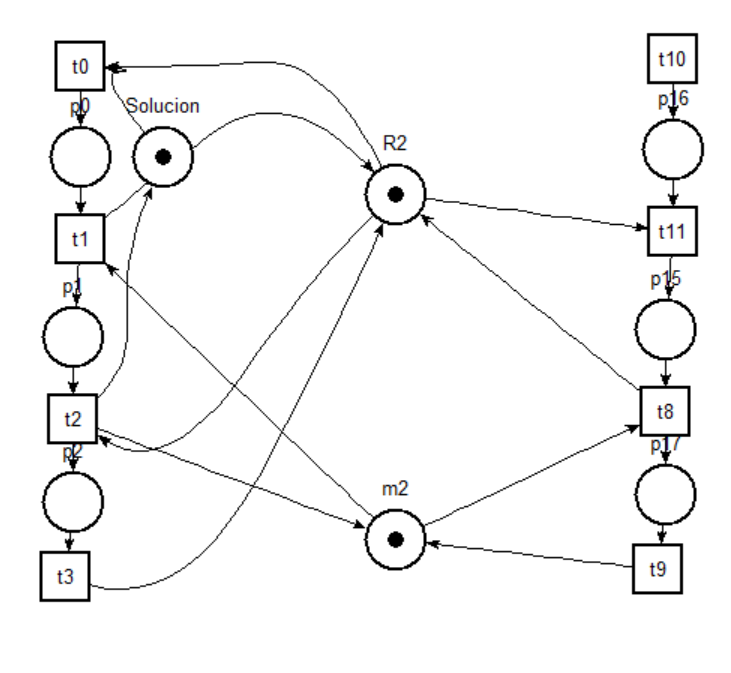
\includegraphics[width=0.4\linewidth]{./figure/I20}}
	{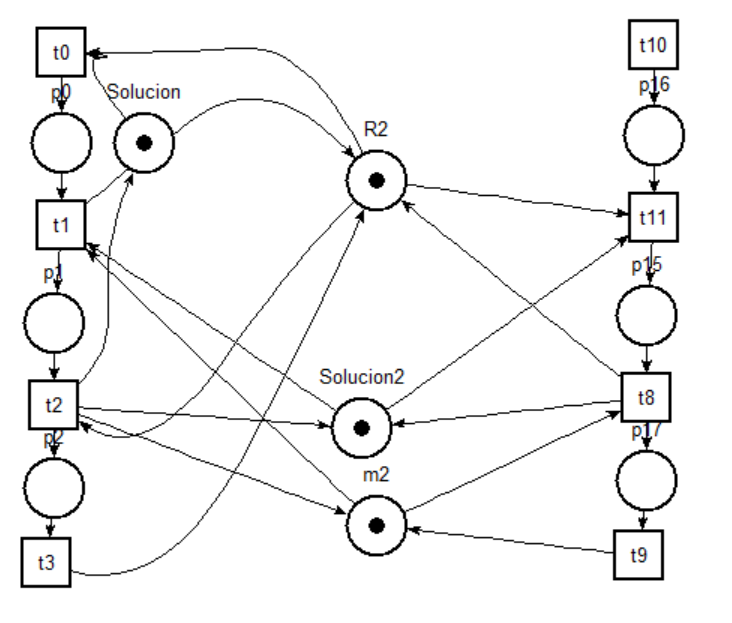
\includegraphics[width=0.4\linewidth]{./figure/I21}}
	\caption{Esquema simplificado del segundo problema de interbloqueo.}
	\label{fig:I20}
\end{figure}

Plaza 3:
En este caso es encontró que la linea de producción de la pieza C era la misma que una de las alternativas de la pieza A, por lo tanto la única solución a este conflicto es agregar una restricción que no permita que ambas lineas produzcan al mismo tiempo. 

\begin{figure}[H] % Example image
	\centering{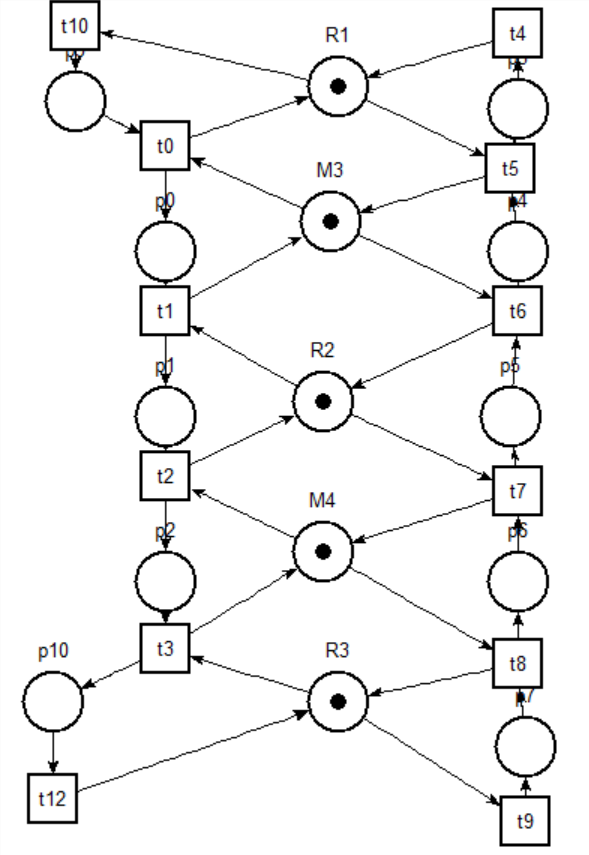
\includegraphics[width=0.4\linewidth]{./figure/I30}}
	{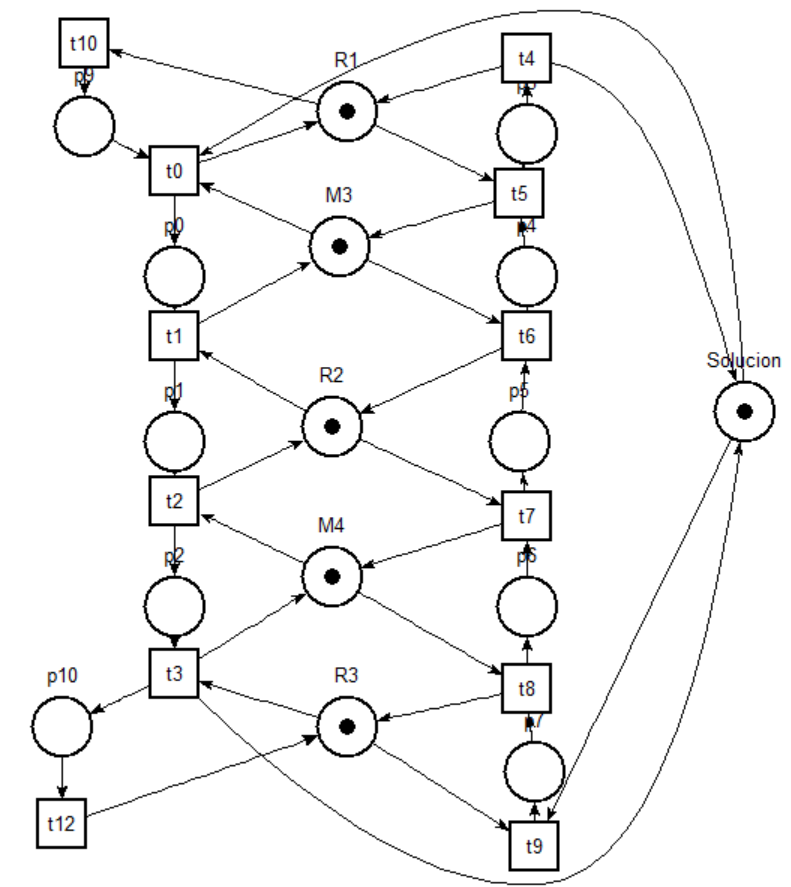
\includegraphics[width=0.4\linewidth]{./figure/I31}}
	\caption{Esquema simplificado del tercer problema de interbloqueo.}
	\label{fig:I30}
\end{figure}

Como resultado se obtiene la siguiente red, se puede comprobar con el software PIPE que no posee interbloqueo.

\begin{figure}[H] % Example image
	\centering{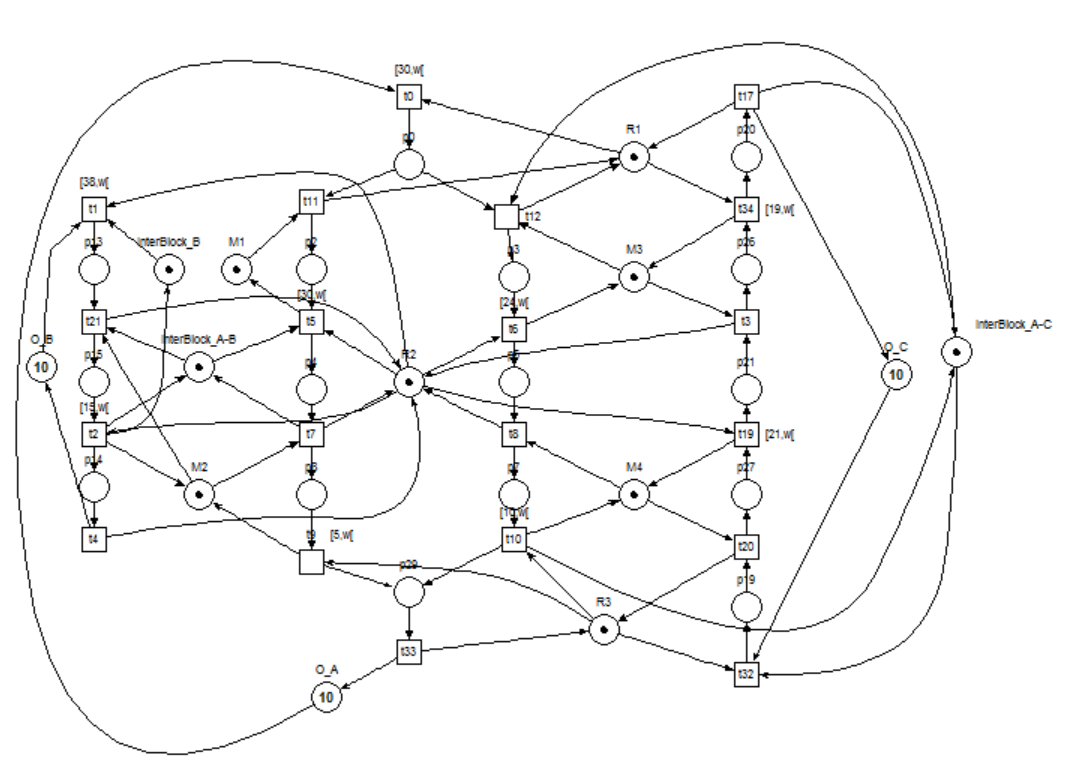
\includegraphics[width=1\linewidth]{./figure/Red01.png}}
	\caption{Red con problemas de interbloqueo solucionado.}
	\label{fig:red}
\end{figure}


En la figura también se incluyen los tiempos asociados a las transiciones, según se indico en el enunciado. También se debieron agregar tiempos adicionales a algunas transiciones para equilibrar la producción de piezas de distintos tipos.

Una vez construida y verificada la red, se procede al desarrollo de un programa que pueda simular su comportamiento.



\section{Implementación de un monitor con Red de Petri}
%que es un monitor??
\subsection{Clases}
Con el objetivo de modularizar el código y procurar el desacoplo de cada parte, se decidió la implementación de las siguientes clases:

\begin{itemize}
	\item Main
	\item Rdp
	\item GestorMonitor
	\item Politicas
	\item Colas
	\item Mutex
	\item Tiempo
\end{itemize}

Se muestra a continuación el diagrama de clases y luego se desarrollará una breve descripción de las clases más importantes y se detallan los métodos más relevantes
\begin{figure}[H] % Example image
	\centering{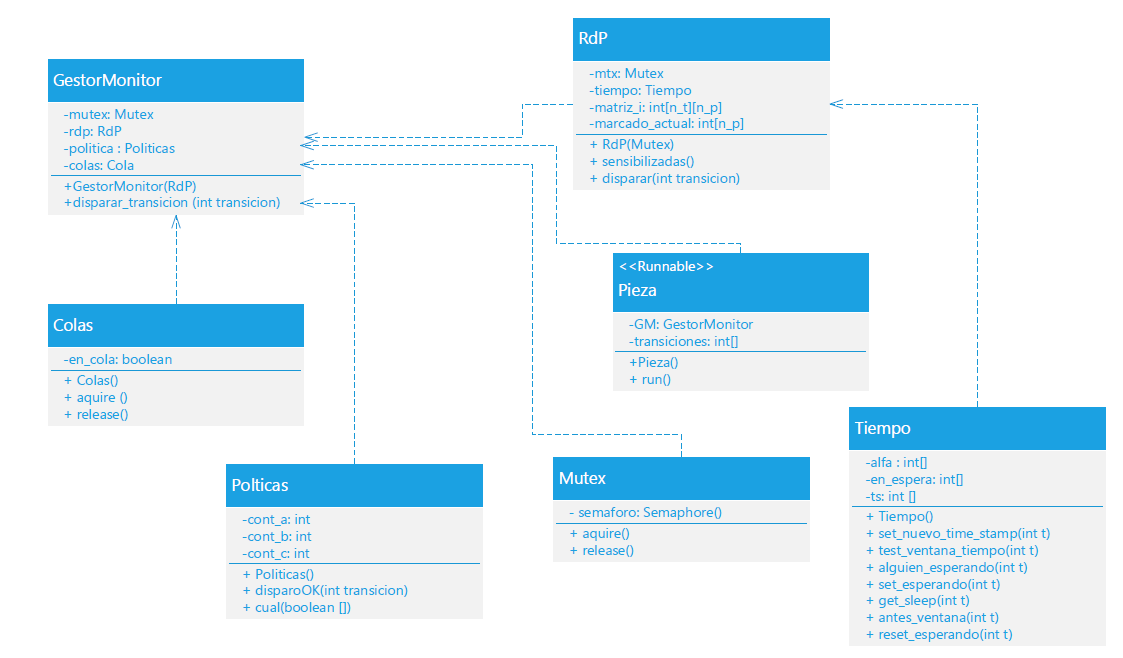
\includegraphics[width=1\linewidth]{./figure/clases.png}}
	\caption{Diagrama de clases de un monitor.}
	\label{fig:clases}
\end{figure}

\subsubsection{Main}
Se inicializa el gestor de monitor pasando los parámetros necesarios y los 5 hilos que ejecutaran sus correspondientes transiciones.

\subsubsection{Rdp}
Contiene toda la lógica del monitor, es decir controla la exclusión mutua y administra los recursos disponibles. De este modo esta clase contiene las matrices de incidencia pre y pos, y el vector de marcado; estas variables combinadas representan el estado de la red en un momento determinado. \\
Entre sus funciones mas relevantes se encuentran:

\begin{itemize}
	\item \textit{Sensibilizadas():} devuelve un arreglo de boolean que representa las transiciones sensibilizadas en un momento determinado. Este vector se calcula sumando el vector de marcado actual a la matriz de incidencia I, una vez realizada esta operación, se controla que en la columna correspondiente a una transición no existan elementos negativos. Si existe un valor negativo para una plaza en la columna de una transición, esta transición no esta sensibilizada; en el caso contrario, la transición esta sensibilizada.
	\item \textit{Disparar():} realiza(en el caso que sea posible) el disparo de la red y devuelve un entero indicando el resultado del disparo. El disparo se realiza con la ecuación de estado de la Red de Petri:
	\begin{equation*}
	m_{n+1} = m_n + I \times d_j
	\end{equation*}
	donde $ m_{n+1} $ es el marcado en el instante n+1, $m_n$ el marcado en el instante n, $I$ la matriz de incidencia y $d_j$ el vector de disparo para una transición j.\\
	Una vez calculado el resultado del disparo de una transición se hace el cheque de tiempo, por medio de los métodos de la clase Tiempo
	
\end{itemize}

\subsubsection{GestorMonitor}
En esta clase se encarga de la gestión de hilos después de un disparo, tiene un solo método que es disparar transición, en el cual el hilo debe acceder al gestor por medio de un mutex de entrada. De este modo el gestor se asegura que solo un hilo pueda disparar la red a la vez.
\\
Una vez realizad el disparo pueden ocurrir varias alternativas, el hilo puede haber disparado la transición correctamente, entonces el gestor le da la señal al hilo para que dispare la próxima transición. Luego existen varios casos en los que no se puede disparar la transición y según la situación el hilo puede irse a una cola FIFO, dormirse o simplemente salir del monitor para nuevamente intentar disparar la misma transición.
\\
Si un hilo realiza un disparo, si hay otros hilos en las colas del gestor deberá despertarlos, si hay mas de un hilo en las colas y con sus respectivas transiciones sensibilizadas se acudirá a la clase política para decidir cual disparar.
\\
La imagen a continuación es un diagrama de secuencias que permite explicar el funcionamiento del gestor de monitor sin tiempo:

\begin{figure}[H] % Example image
	\centering{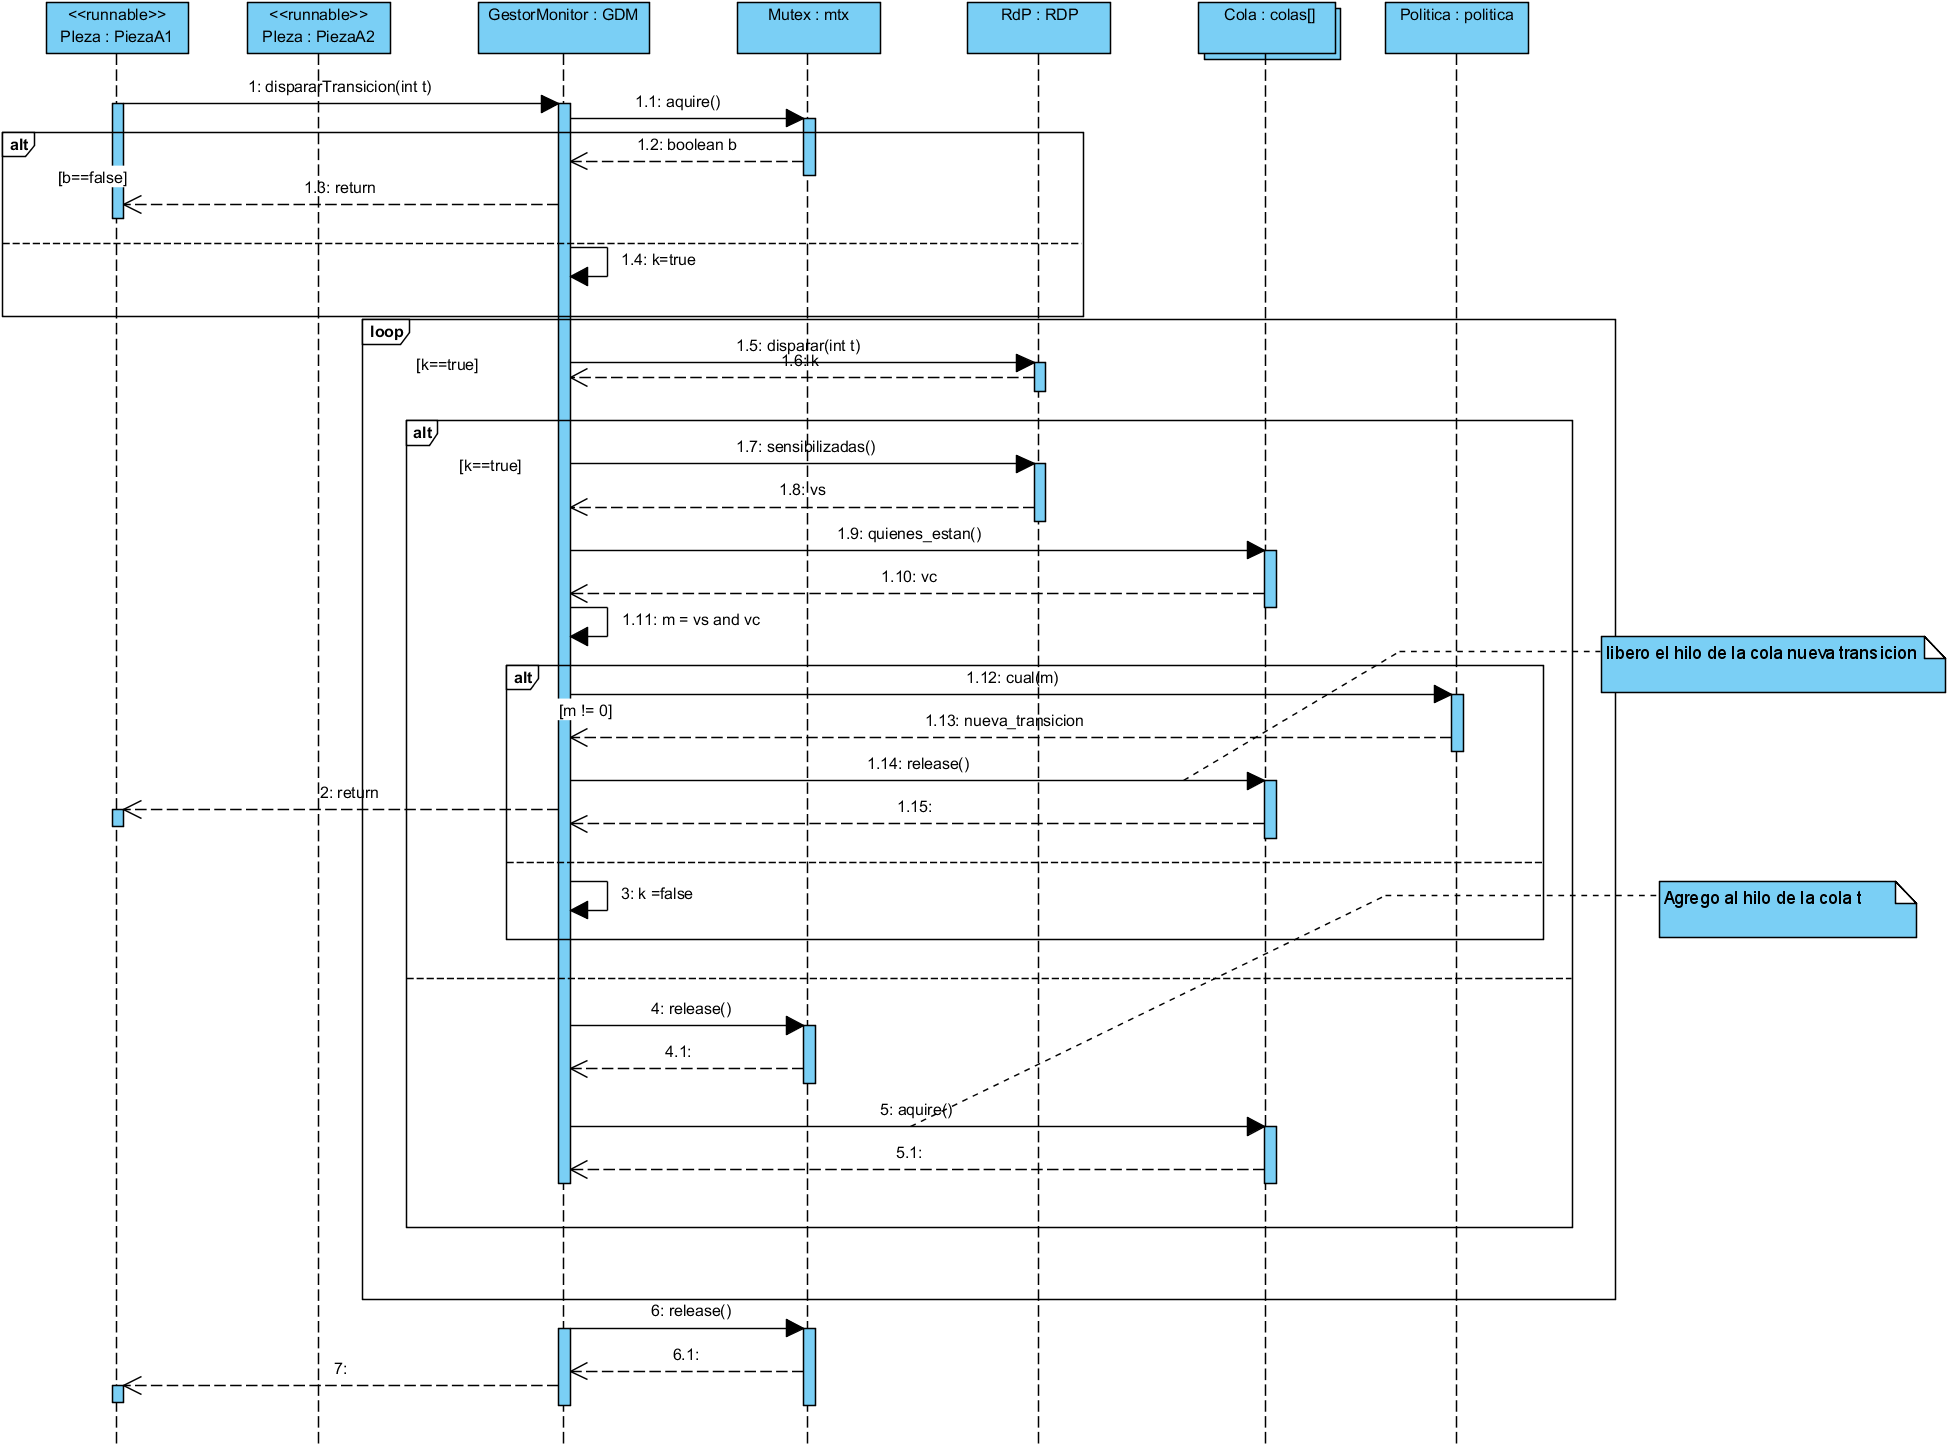
\includegraphics[width=1\linewidth]{./figure/GestorDeMonitor.png}}
	\caption{Diagrama de secuencia de disparo de una transición sin tiempo.}
	\label{fig:sec}
\end{figure}

\subsubsection{Politicas}
Esta clase es la que toma la decisión de que transición disparar en el caso en que haya dos o mas transiciones sensibilizadas y con hilos en sus colas. Lleva contadores que se actualizan en cada disparo, cuentan la cantidad de piezas terminadas de cada tipo y como parámetro tiene las proporciones de producción de cada pieza. Los métodos mas relevantes son:
\begin{itemize}
	\item Cual(): se ele pasa un vector con las transiciones sensibilizadas y devuelve la transición que se debe disparar. Se calcula multiplicando el vector por una matriz que lo ordena según la prioridad actual de producción de piezas
	\item ActualizarP(): actualiza la matriz que ordena el vector según la cantidad de piezas producidas.
\end{itemize}
\subsubsection{Cola}
La colas tienen un papel importante en el desarrollo de software concurrente aplicado a una red de petri. Las colas son las encargadas de establecer un "fila" para los hilos que esperarán a disparar una transición determinada.
Es por esto que cada transición de la red tendrá asociado un objeto de esta clase, la misma contendrá dos métodos:
\begin{itemize}
	\item acquire(): el hilo ejecutor de este método se va a "dormir" a la cola (que en estado interrumpido) hasta la ejecución del release de esta clase
	\item release(): despierta el hilo dormido en la cola
\end{itemize}

\subsubsection{Mutex}
El mutex es la "puerta de entrada" al monitor. Todo hilo que busque ejecutar una acción dentro del programa deberá "pedir autorización" para entrar.
Esta clase utiliza un Semaphore de la librería java.util.concurrent. El mismo posee una cola de los hilos que buscan entrar al monitor,
\subsubsection{Tiempo}
Este objeto es el que almacena los tiempos de sensibilización de cada transición y los retrasos asociados a algunas transiciones. Algunas de sus funciones son:
\begin{itemize}
	\item TestVentanaTiempo(): 
\end{itemize}
El diagrama a continuación representa el calculo de un disparo con tiempo
\begin{figure}[H] % Example image
	\centering{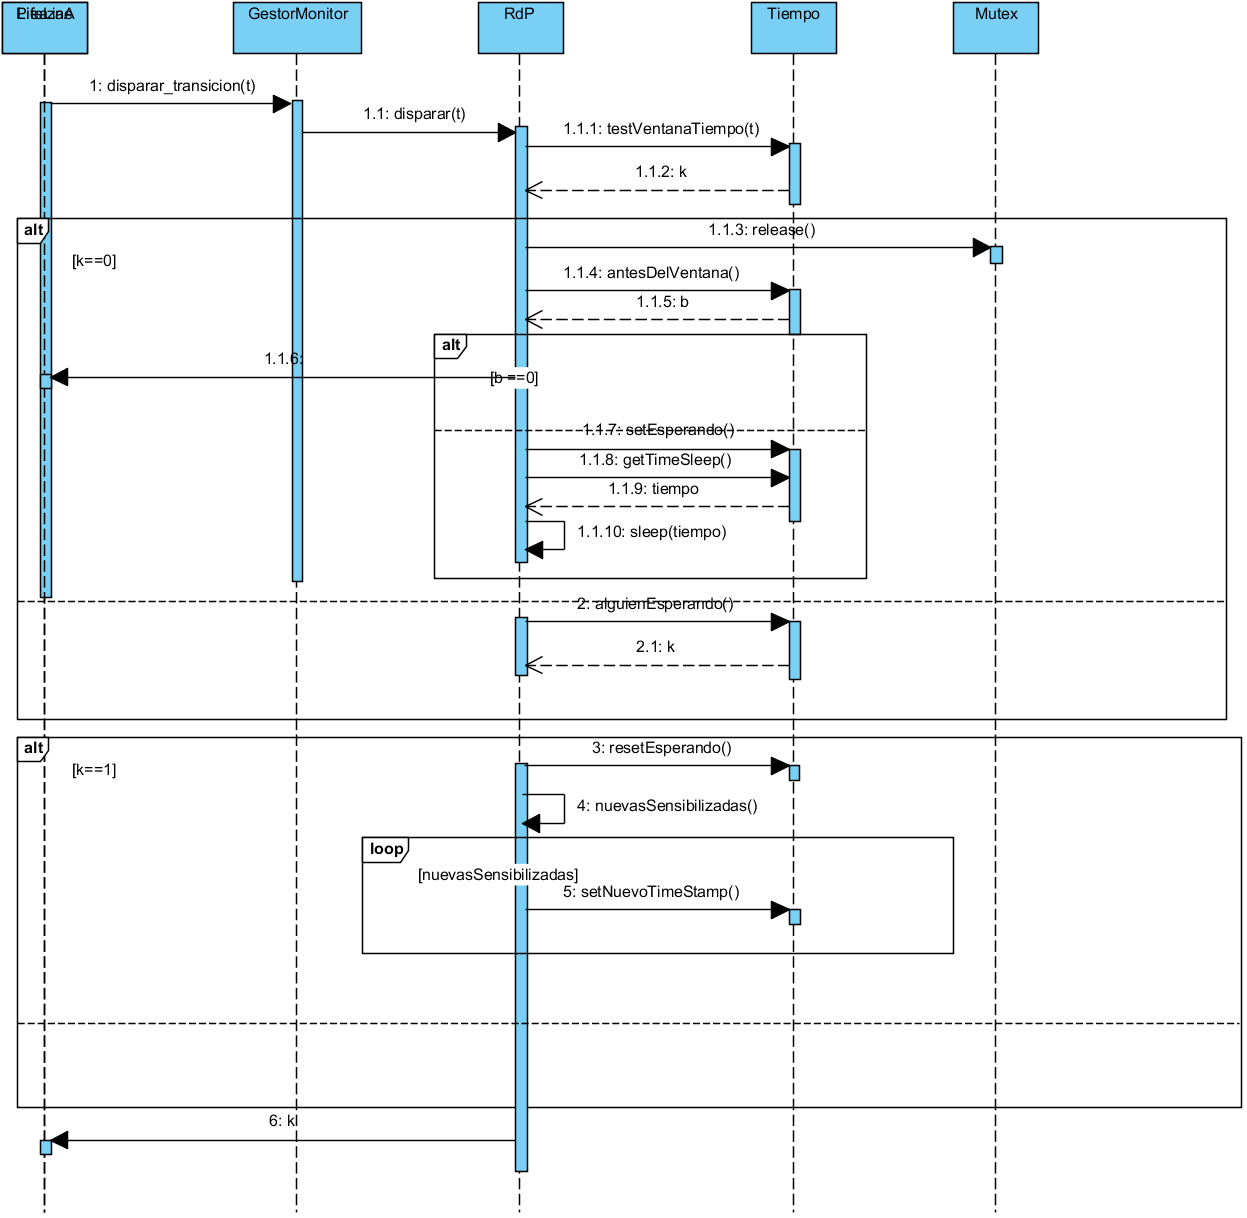
\includegraphics[width=1\linewidth]{./figure/sec_tiempo.png}}
	\caption{Diagrama de secuencia de disparo de una transición con tiempo.}
	\label{fig:sec2}
\end{figure}

\section{Pruebas y Testing}
En todo sistema automático y con secciones criticas, es necesario brindar la seguridad de que el sistema realizar perfectamente las acciones asociadas al mismo.
Cabe destacar los fundamentos matemáticos proveídos por las Redes de Petri para este tipo de prueba, como son las P-Invariante. Estos asegurar el correcto funcionamiento de la lógica en el software.
\subsection{Unit Test Java}
Se generaron dos test unitarios de java para probar el método de disparar transición del objeto Rdp, con la finalidad de corroborar la lógica del programa. En las pruebas se utilizaron dos redes de petri diferentes, una la que corresponde a nuestro caso y la otra una red sencilla. En este caso se utilizó un productor/consumidor.\\
Para verificar que los disparos se produjeran correctamente y respetando la lógica de la red, estos test se hicieron probando las P-Invariante proporciondas por el software PIPE. Esta prueba garantiza que después de cada disparo el marcado de la red sea coherente con la lógica que representa.
% Acá irá una captura del resultado del test

\begin{thebibliography}{100} % 100 is a random guess of the total number of
%references

Agregar bibliografía.

el libro de java del práctico

filminas de clase

diagramas desecuencia del profe

se puede poner wel paper de mico (el tipo sabe q esta en interenet y por ende sabe q tenesmo acceso, no es boludo. quedariamos bien admitiendo que lo usamos. de paso le chupamos un toque las medias)

etc


\end{thebibliography}


\end{document}